\section{Déploiement}
\label{sec:deployment}

\subsection{Architecture de l'application}

Une application de démonstration a été développée pour illustrer
concrètement le comportement des deux modèles. Elle repose sur une
architecture client-serveur classique :

\begin{itemize}
  \item \textbf{Backend} (FastAPI) : expose trois endpoints REST -
    \texttt{/predict} (prédictions ViT et ResNet-50 avec confiance et
    top-3), \texttt{/attention} (carte d'attention du ViT superposée à
    l'image), et \texttt{/classes} (noms des 200 espèces). Les modèles
    sont chargés une seule fois au démarrage du serveur, à partir des
    checkpoints entraînés (Section~\ref{sec:methodology}), pour une
    inférence CPU en temps quasi réel sur une image à la fois.
  \item \textbf{Frontend} (Next.js) : interface d'upload par
    glisser-déposer, affichage comparatif des deux modèles côte à côte
    avec barres de confiance, indicateur visuel d'accord ou de désaccord
    entre les deux architectures, et superposition de la carte
    d'attention sur l'image d'origine.
\end{itemize}

\subsection{Extraction de la carte d'attention}

La carte d'attention du ViT est obtenue en interceptant, via un hook
PyTorch, les poids d'attention du dernier bloc Transformer entre le
token \texttt{[CLS]} et les patches de l'image (moyennés sur les têtes
d'attention), puis en les redimensionnant à la taille de l'image
originale pour former une heatmap superposée.

\subsection{Exemples d'utilisation}

La Figure~\ref{fig:app_nominal} illustre un cas nominal : une image du
jeu de test (\emph{Gray-crowned Rosy Finch}) est correctement identifiée
par les deux modèles, avec un fort accord (ResNet-50 : 83{,}4\,\% de
confiance ; ViT : 26{,}5\,\%).

La Figure~\ref{fig:app_ood} illustre un cas hors distribution : une
photographie de rouge-gorge européen, une espèce absente de
CUB-200-2011, est soumise à l'application. Les deux modèles produisent
des prédictions à faible confiance et sont en désaccord l'un avec
l'autre, ce qui constitue un signal cohérent d'incertitude plutôt qu'une
erreur silencieuse - un comportement souhaitable pour une application
destinée à un usage réel.

\begin{figure}[t]
  \centering
  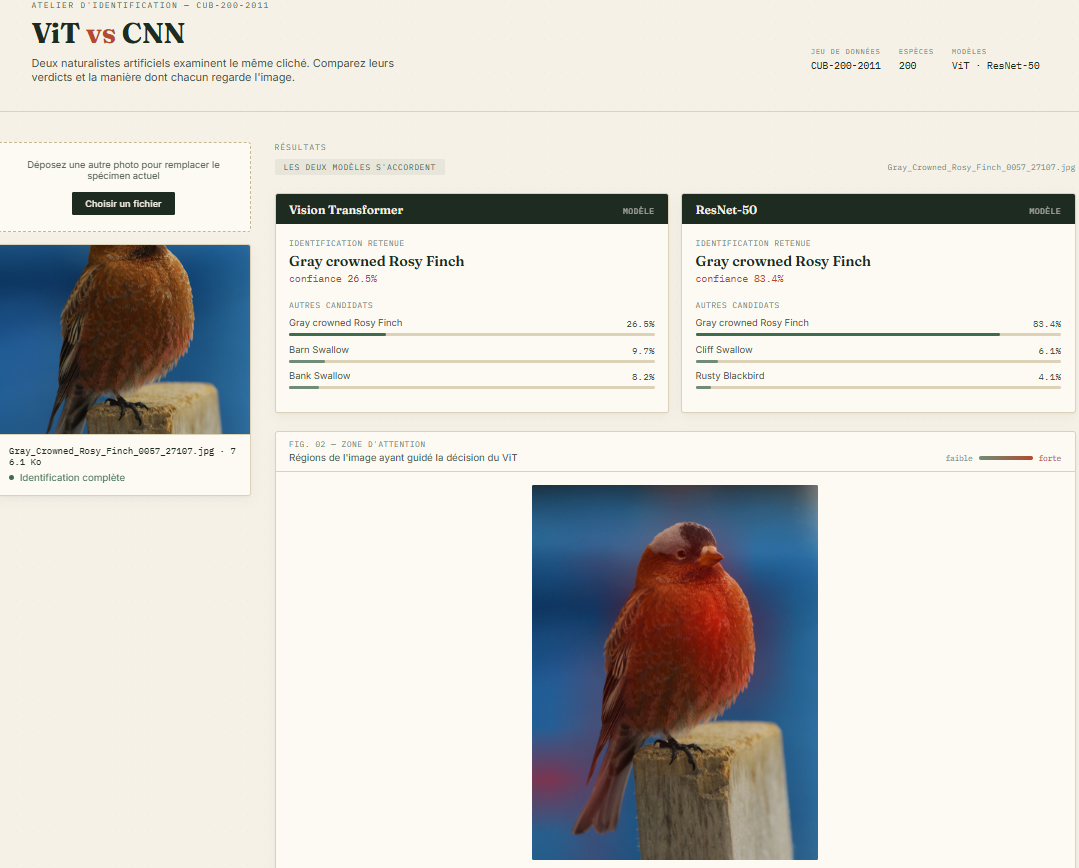
\includegraphics[width=\linewidth]{figures/app_nominal.png}
  \caption{Cas nominal : identification correcte et accord entre les deux modèles sur une image du jeu de test CUB-200-2011.}
  \label{fig:app_nominal}
\end{figure}

\begin{figure}[t]
  \centering
  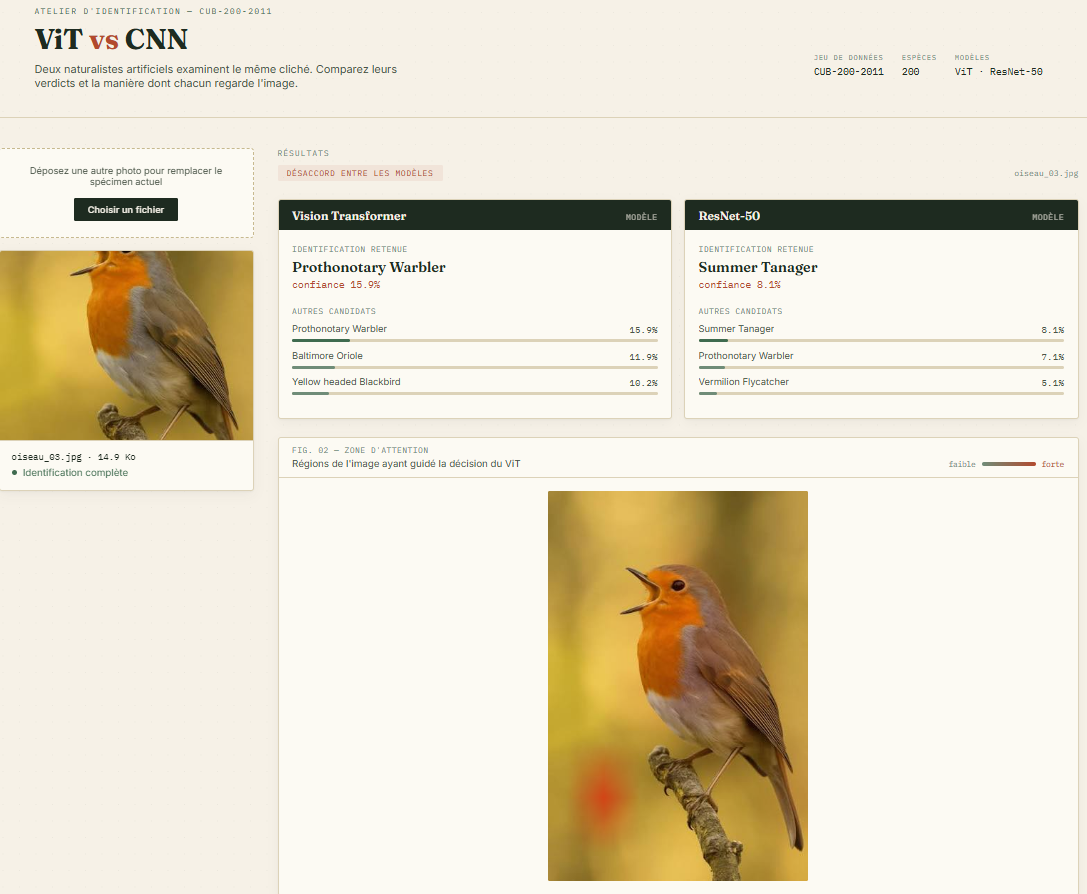
\includegraphics[width=\linewidth]{figures/app_ood.png}
  \caption{Cas hors distribution : une espèce absente du jeu d'entraînement (rouge-gorge européen) produit de faibles confiances et un désaccord entre les modèles.}
  \label{fig:app_ood}
\end{figure}